\documentclass{tufte-handout}

\title{On ultimate; O1: primary middle, focus or left wing}
\author[James Reynolds]{James Reynolds}

%\date{28 March 2010} % without \date command, current date is supplied

%\geometry{showframe} % display margins for debugging page layout

\usepackage{graphicx} % allow embedded images
  \setkeys{Gin}{width=\linewidth,totalheight=\textheight,keepaspectratio}
  \graphicspath{{graphics/}} % set of paths to search for images
\usepackage{amsmath}  % extended mathematics
\usepackage{booktabs} % book-quality tables
\usepackage{units}    % non-stacked fractions and better unit spacing
\usepackage{multicol} % multiple column layout facilities
\usepackage{lipsum}   % filler text
\usepackage{fancyvrb} % extended verbatim environments
  \fvset{fontsize=\normalsize}% default font size for fancy-verbatim environments

% Standardize command font styles and environments
\newcommand{\doccmd}[1]{\texttt{\textbackslash#1}}% command name -- adds backslash automatically
\newcommand{\docopt}[1]{\ensuremath{\langle}\textrm{\textit{#1}}\ensuremath{\rangle}}% optional command argument
\newcommand{\docarg}[1]{\textrm{\textit{#1}}}% (required) command argument
\newcommand{\docenv}[1]{\textsf{#1}}% environment name
\newcommand{\docpkg}[1]{\texttt{#1}}% package name
\newcommand{\doccls}[1]{\texttt{#1}}% document class name
\newcommand{\docclsopt}[1]{\texttt{#1}}% document class option name
\newenvironment{docspec}{\begin{quote}\noindent}{\end{quote}}% command specification environment

\begin{document}

\maketitle% this prints the handout title, author, and date



%\printclassoptions
This document is about 
playing primary 'middle', 
the focus, 
or left wing 
on offence,
referred to here 
as position O1\footnote{This
is part of a series, 
available at
\url{https://github.com/James-Reynolds/Ultimate-strategy-and-tactics}}.
You are starting the point on offence. 
Let the handlers 
deal with catching the pull, but
as you run downfield
try to 
see
what defence structure
is being used. 
%\footnote{It could be:
%person-match defence,
%person-match-last-back-helps,
%person-match-with-a-poacher,
%person-match-with-lots-of switching,
%force-middle,
%force-straight-up,
%zone-3-3-1-force-middle-
%zone-3-3-1-force-sideline
%zone-3-3-1-force-forehand
%zone-3-3-1-force-backhand
%zone-3-3-1-etc
%zone-3-2-2, 
%zone-2-3-2, 
%zone-1-3-2-1 (puppy-fence),
%clam,
%or something else}.

\section{Beating person-match defence with a vertical stack}\label{sec:vertical}

\begin{marginfigure}%
  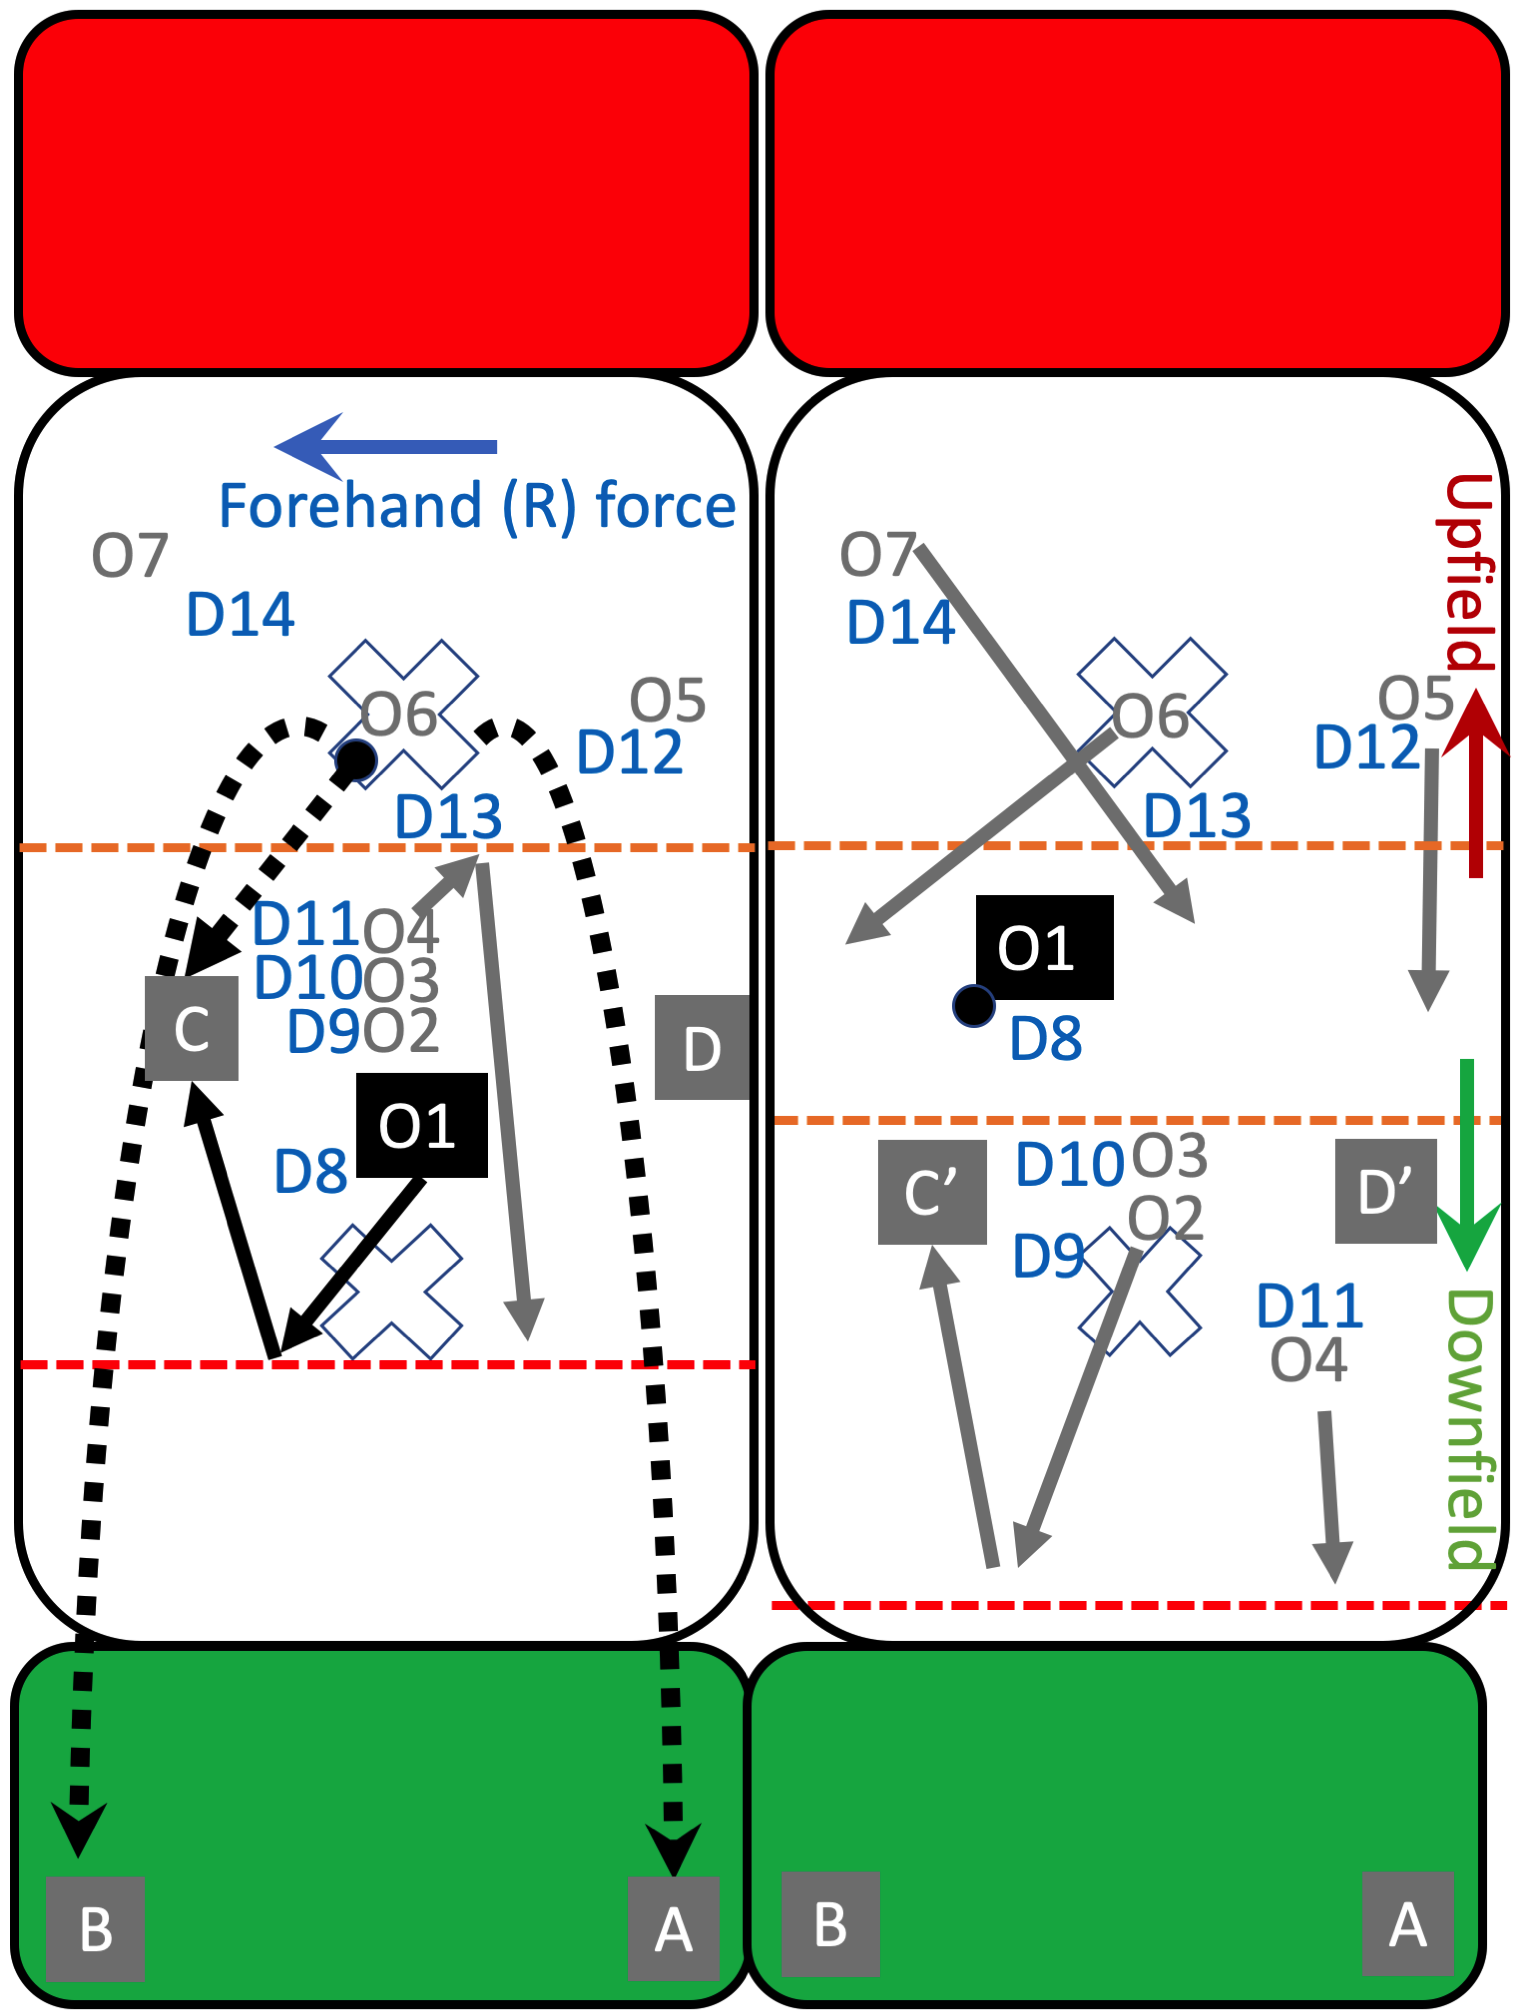
\includegraphics[width=\linewidth]{O1-vertical}
  \caption{Vertical stack: 
  starting position (left),
  and development (right)}
  \label{fig:O1-vertical}
\end{marginfigure}


Figure \ref{fig:O1-vertical} (left) shows 
how everyone might 
setup 
if there is: 
a brick called;
a forehand force; 
person-match defence; 
and your team has decided to use 
a vertical stack formation.
Restricting your cutting 
to between 
the dashed 
horizontal 
lines 
can help\footnote{
Position of 
the dashed red line might vary
with how far O6 
can or will 
throw. 
If you go 
downfield of the dashed red line 
before the disc is in the air,
D8 may be able 
get to
A or B 
before the disc,
intercepting 
or preventing 
deep throws to 
you or others. 
Similarly, 
if you go 
upfield of the dashed yellow line
then D8 may 
be able to help
prevent dump throws from O6
to O5 
or O7.
Hence,
if you cut to C
but the disc is not thrown to you
perhaps cut deep 
to clear the area, 
then return to the stack
and make space for O2-O4}. 

In Figure \ref{fig:O1-vertical} (left)
O6 is shown
potentially throwing 
you (O1) either:
\begin{enumerate}
\item A break-side 
huck to A.
This throw is 
probably 
difficult. 
However, you as O1
can just
stand still 
till O6 throws it, 
then run and catch it.
Figure \ref{fig:O1-vertical} indicates how 
D8 will be on the wrong side of you
and so probably 
be able to get to the disc
first.
\item An open-side huck to B. 
This is viable if: 
D8 is closer to the disc than you; 
you are faster than D8; or 
D8 does not cover 
an initial cut downfield (black arrow). 
\item A throw 
to C.
The solid black arrows indicate 
a cut you might do;
initially going deep,
but then coming back-under
on the open side. 


\item A break throw to D. 
Any of the cutters 
(O1-4)
can go and catch this, 
as all the defenders 
(D8-D11) 
are on the wrong side
However,
if anyone 
except O4 
cuts towards D 
\smallcaps{prior to the disc being thrown} 
then there is likely 
to be a pick\footnote{
Picks are
when a defender 
cannot follow 
someone they are marking.  
However, 
once the disc is thrown,
everyone can move anywhere 
to try and catch it. 
So, maybe stand still 
until it's thrown 
to avoid a pick}.
\end{enumerate}

Figure \ref{fig:O1-vertical} (right) shows 
the disc having been thrown to you
on the back-under cut towards C. 
In order of desirability, 
your options may include: 
(1)
off-load to O6, 
putting them in power position;
(2) throwing to A' to hit O2 or O4;
(3) throwing to B' or C' for O2;
(4) break force throw 
to centre the disc
to O3 or O5;
(5) dump to O7.
Then, head back to the stack, 
or make another cut.

Vertical works
against other person-match defences. 
But it might need 
some adjustment.
For example:
against (1) RH-backhand-force: mirror the above;
against (2) person-match-straight-up-force:  
your defender (D8) 
may just cover you under,  
so maybe
stand at the back of the stack
until one of the handlers 
have a chance to throw 
(deep)
without a marker.


\subsection{Beating person-match defence with feldrunner}
\label{sec:feld}
\begin{marginfigure}%
  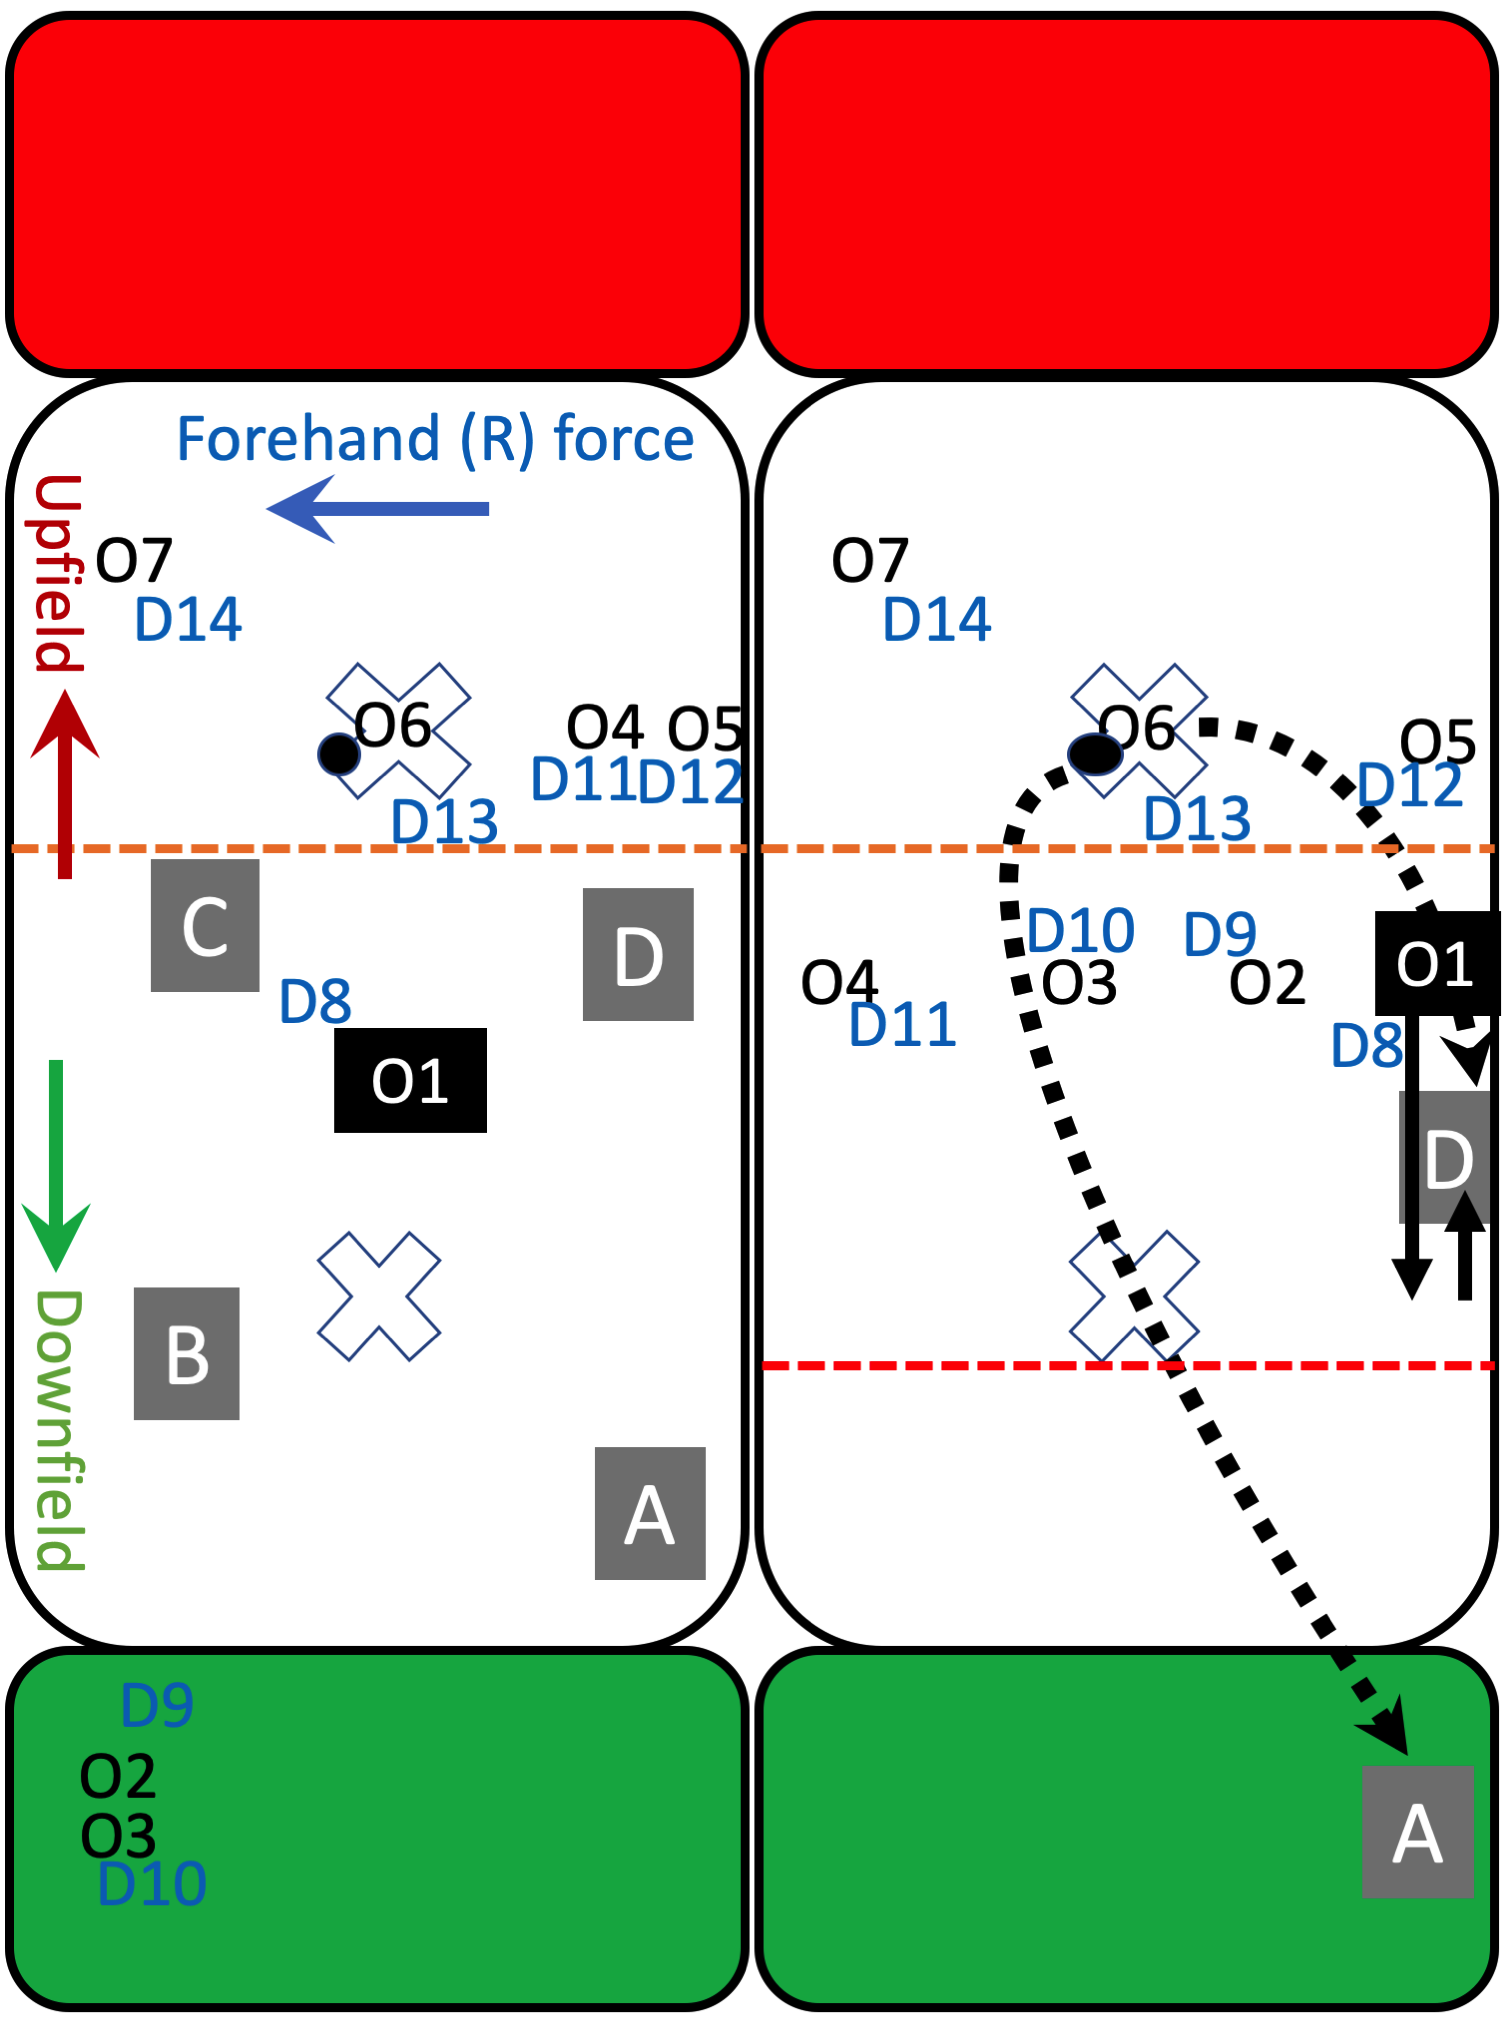
\includegraphics[width=\linewidth]{O1-horizontal}
  \caption{Feldrunner (left) and horizontal (right)}
  \label{fig:O1-horizontal}
\end{marginfigure}

Figure \ref{fig:O1-horizontal} (left) 
shows a feldrunner formation, 
with 4 handlers
and 2 cutters
in a
stack in the endzone.
It involves 
leaving you 
(O1) 
isolated 
in the centre
as the focus. 
O6 can throw 
to A,
B, 
C 
or D. 
If D8 looks at you, 
let O6 throw it first. 
If D8 is 
looking at O6, 
make a cut. 
It might get dumped 
but then it just resets with 
one of O4, O5 or O7, 
trying to throw to you.
Once you get the disc 
either throw a goal 
to a cut 
from O2-3, 
or dump to 
one of O4-7 
and repeat. 


\subsection{Beating person-match defence with a horizontal stack}\label{sec:horizontall}
Basic horizontal stack 
involves cutting
upfield and downfield (black arrows)
within your quarter of the field\footnote{
Other cuts
can work, 
but might need
communication,
e.g. diamond cuts 
involve you trading places 
with O2.}. 
Figure \ref{fig:O1-horizontal} (right) shows 
O1 on the left wing. 
O6 
can potentially 
throw to you 
at A 
or D\footnote{
Black arrows
show how a back-under cut 
opens space 
for this throw.}. 
However, 
O6 throwing to 
O2, O3 or O4  
may be easier. 
Hence,  
you may wish to 
wait and 
cut later. 
If you do get the disc 
at D 
a huck to 
A for O2 or 
to B for O4 
may be effective.
Otherwise, 
get it to the middle of the field 
with a dump to O5 or O6. 

A typical pattern
is that D8 (marking you)
will try to help 
D9, D10 and D11 
by poaching deep.
To beat this 
you can: 
trade spots with O5;
move to the open side, 
between D10 and O6; or 
stay still 
on the left wing,
so O6 can 
get it to you 
quickly
with a hammer 
or blade.

\section{Beating zone defence}\label{sec:zone}

\begin{marginfigure}%
  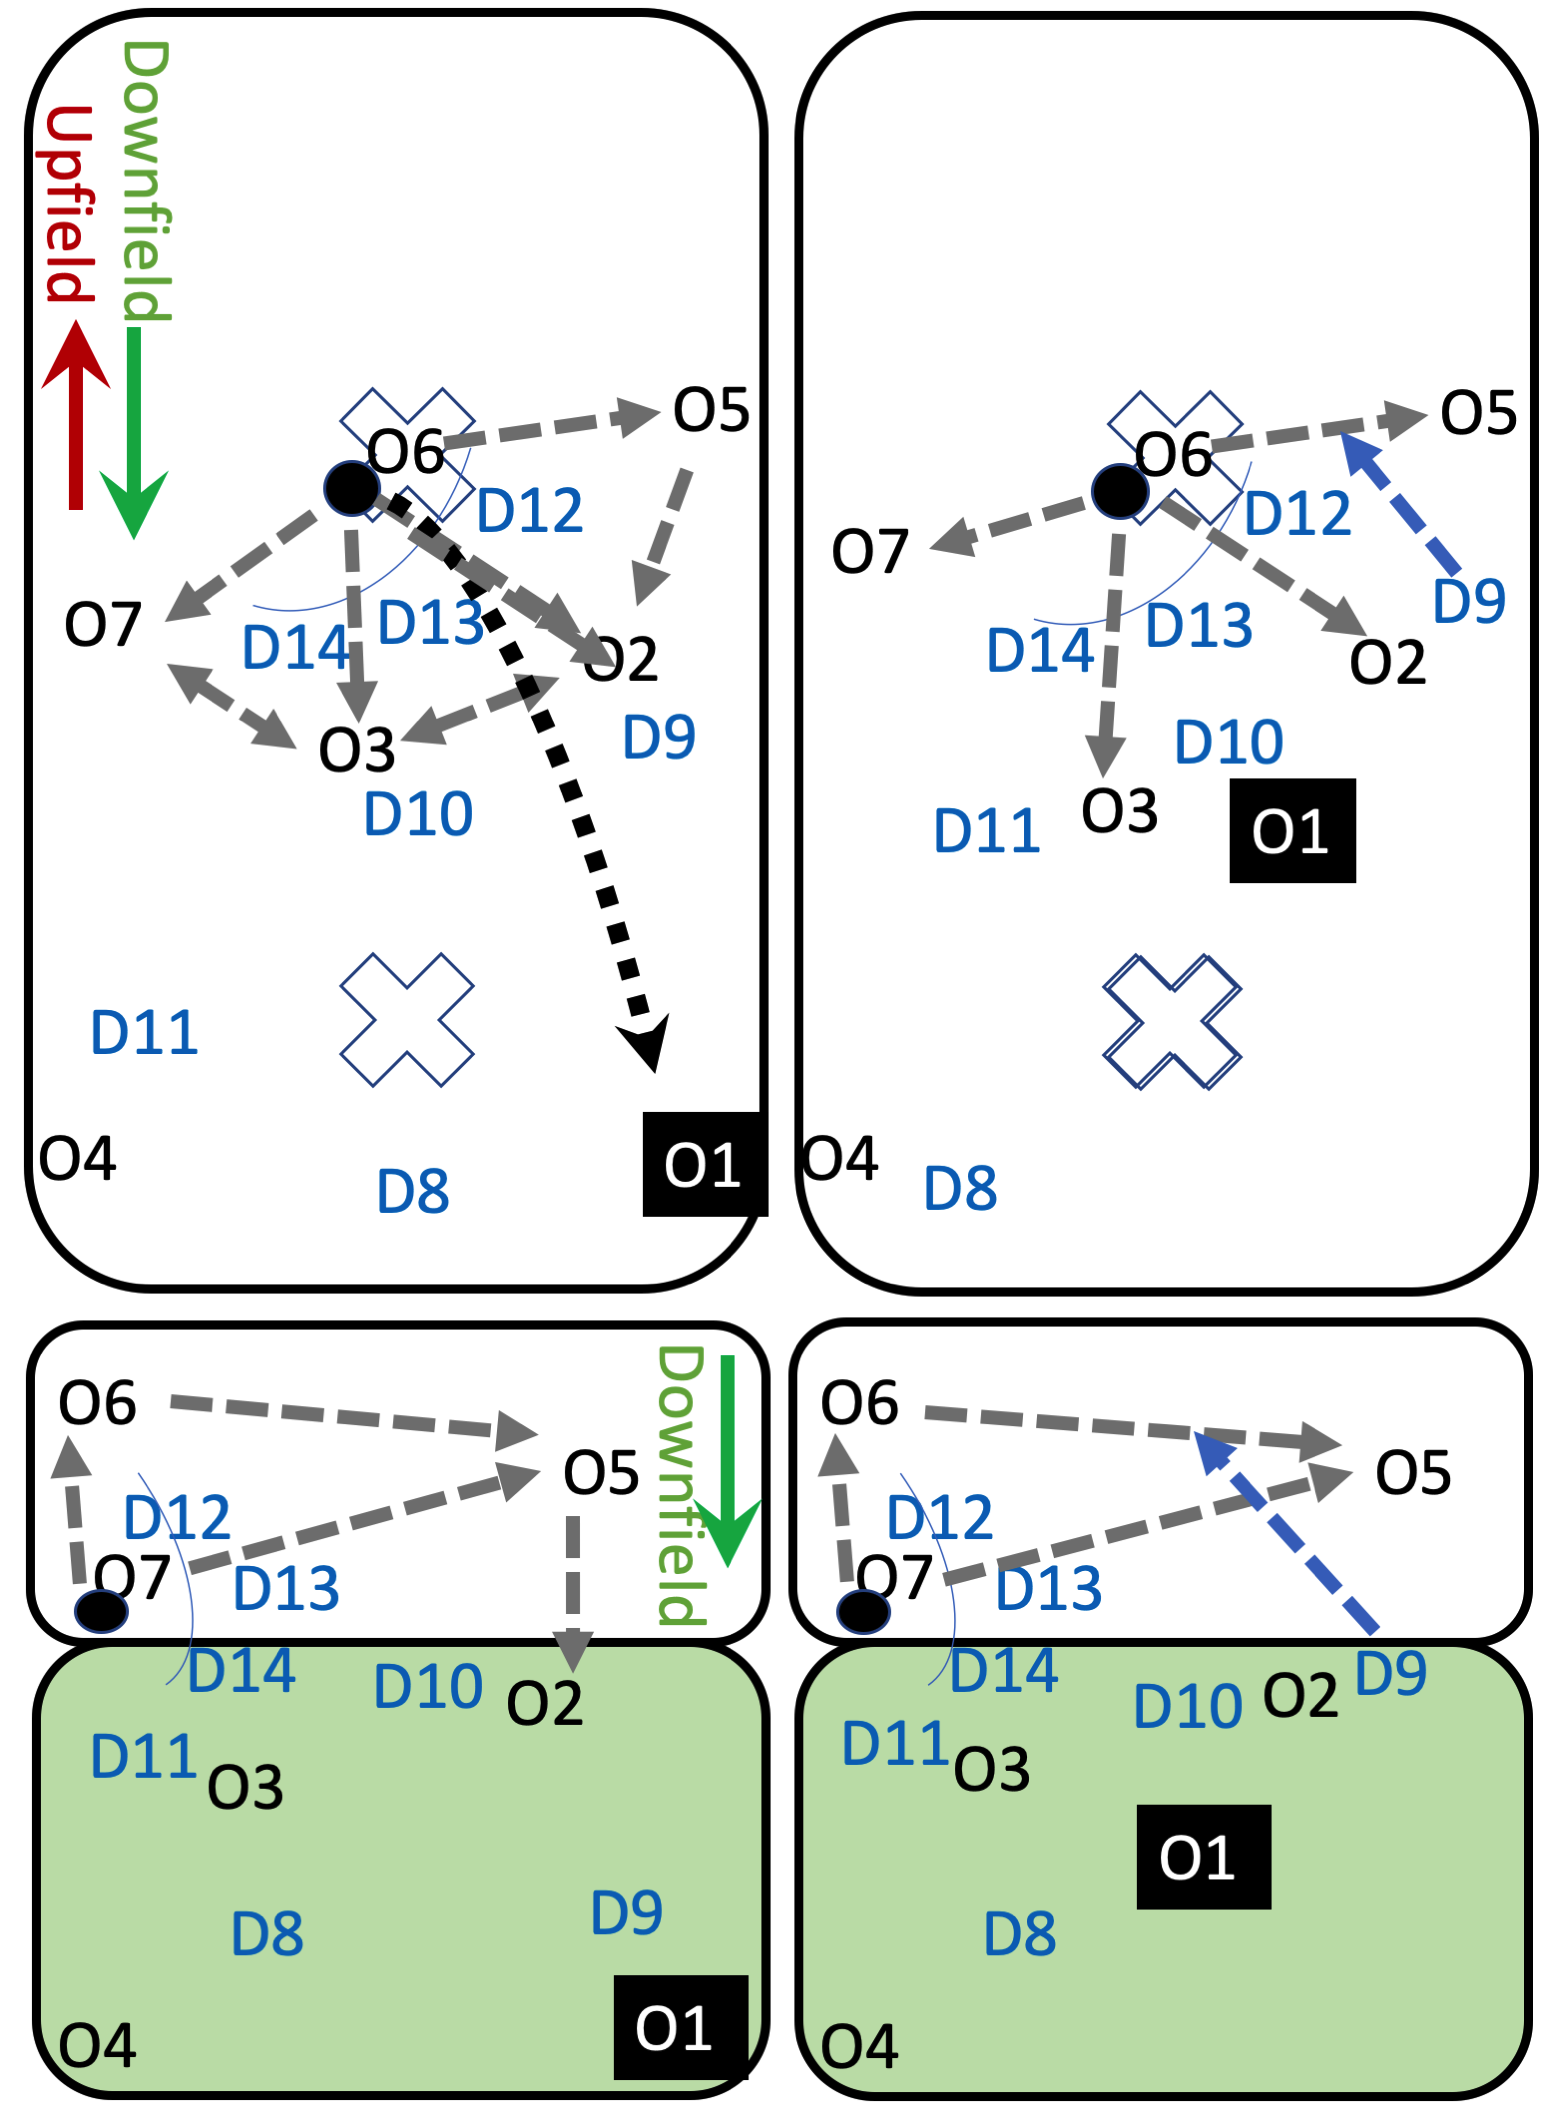
\includegraphics[width=\linewidth]{O1-zone331}
  \caption{effective formations against 331 zone: 
  general (top left)
  and close to the endzone (bottom left); and 
  less effective formations (top, bottom right)}
  \label{fig:O1-zone331}
\end{marginfigure}

Vertical stack 
probably won't work. 
Instead, your 
team needs to 
spread out. 
Three ways to beat a zone are:
(1) over;
(2) round; or
(3) through. 
Figure \ref{fig:O1-zone331}
(top left)
shows this 
against a 
3-3-1 zone. 
As O1 
(left wing), 
you are mostly relevant to 
(1) \smallcaps{over}, 
in the gap between 
D8 
and D9.
Figure \ref{fig:O1-zone331} (top left)
shows a throw 
direct 
from O6 
to you\footnote{
Blade or
hammer 
to get it 
to you
as quickly as possible, 
so may help to 
stand still 
and look at O6.}.
Otherwise, 
O6 might throw
over or through (to O2 or O3), 
or round (to O5 or O7)\footnote{
You, 
O5, 
O2, and
O3 
might then seek to split
D10
and D9,
making ground 
before the cup 
(D12-14) catch up. 
However, 
once the cup arrives, 
it is best to dump to O6, 
so you have 
your 7th player 
downfield.}. 
If the defence 
continues to play zone 
once the disc 
gets close to the endzone, 
you (O1) 
and the other wing (O4) 
can \smallcaps{go and stand 
on the back corners}
(Figure \ref{fig:O1-zone331} (bottom left)\footnote{ 
The defence 
will then have to either 
leave you open
(a direct throw 
(1) over to you then scores)
or cover you
at the corner
(D8 
or D9), 
making more space 
for O2, 
O3, 
O5, 
O6 and
O7 
to score 
at the front of the endzone.}.

Figure \ref{fig:O1-zone331} (bottom right) shows 
how the further 
you are from the back corner 
the more D8/9 
can cover both you
AND others,, 
and the harder 
it is to throw direct to you.
D9 might even be able to get a block
on a throw to O5
(dashed blue line). 
This applies also when 
not close to the endzone 
(top right),
If you crowd O2 and O3,
D8 only has to cover O4, 
and D9-11 get to cover 
you (O1),
O2, 
O3 and 
O5, 
because you are all 
so close together.

\section{Beating clam defense}\label{sec:zone}


\end{document}
